\section{Problem 3}
\label{part3}
\begin{verbatim}
Extra credit, 3 points:
Repeat question #1, but with your LinkedIn profile.
\end{verbatim}
\subsection{Solution}
\begin{enumerate}

\item This question is about determining whether ``Friendship paradox'' holds for LinkedIn account. Here I took ``connections '' as a value of measure to prove the paradox.
\item This is similar to the question 1 and the process of getting LinkedIn data is different and rest of all is the same.
\item Now in order to get LinkedIn data I planned to not use API as it wasted a lot of my time and I was unsuccessful.
\item So, I thought to scrape the data using command prompt and the command to get all my connections is shown in \ref{code1}
\item The sample output for this is shown in \ref{Sample Connections}.
\item My plan was to strip unnecessary data from each of the my connection's link and take them into a csv file.
\item Later on I would run a for loop which takes each connection and get the number of connections they have and store in a file.
\item This gives me the required data and then the same graph,mean,median,mode can be calculated. 
\item I was unable to complete this solution. 

\newpage
\end{enumerate}
\subsection{Commands}
\subsubsection{Comannd to get LinkedIn Connections}
\begin{figure}[ht]    
    \begin{center}
        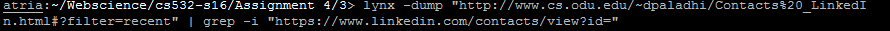
\includegraphics[scale=0.8]{Code_toget_connections.png}
        \caption{Comannd to get LinkedIn Connections}
        \label{code1}
    \end{center}
\end{figure}
\subsection{Results}
\subsubsection{Sample Connections}
\begin{figure}[ht]    
    \begin{center}
        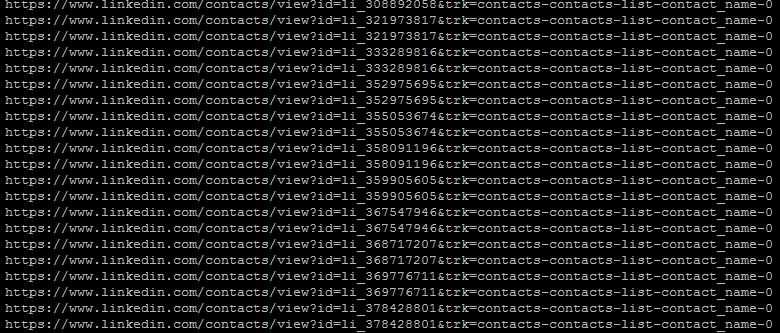
\includegraphics[scale=0.70]{sample_connections.png}
        \caption{Page rank along with 10 URIs}
        \label{Sample Connections}
    \end{center}
\end{figure}

